\RequirePackage{graphicx}
\documentclass{beamer}
\usepackage{blkarray}
\usepackage{enumerate}
\usepackage{caption}
\usepackage{color}
\usepackage{beamerthemesplit}
\usepackage{graphicx}
\usepackage{pdfpages}
%\usepackage{tikz}
\usepackage{epstopdf}
%\usetheme{Antibes}
\DeclareGraphicsExtensions{.tiff, .jpg, .png}
\newcommand{\union}{\bigcup}
\newcommand{\intersect}{\bigcap}
\newcommand{\QED}{\blacksquare}
\newcommand{\homo}{\simeq}
\newcommand{\A}{\big(A_1,\ldots,A_m\big)}
\newcommand*\diff{\mathop{}\!\mathrm{d}}
\newcommand*\Diff[1]{\mathop{}\!\mathrm{d^#1}}
\newcommand{\R}{\mathbb{R}}
\newcommand{\Z}{\mathbb{Z}}
\newcommand{\Q}{\mathbb{Q}}
\newcommand{\N}{\mathbb{N}}
\newcommand{\C}{\mathbb{C}}
\newcommand{\h}{\mathbb{H}}
\newcommand{\T}{\mathcal{T}}
\newcommand{\s}{\mathcal{S}}
\newcommand{\E}{\mathcal{E}}
\newcommand{\F}{\mathcal{F}}
\newcommand{\p}{\mathcal{P}}
\newcommand{\w}{\mathcal{W}}
\newcommand{\ov}{\overline}
\newcommand{\comp}{\overline}
\newcommand{\snd}{\Sigma_{n,d}}
\newcommand{\pnd}{\R[x_1,\ldots,x_n]_{2d}}
\newcommand{\pn}{\R[x_1,\ldots,x_n]}

\DeclareMathOperator{\trace}{trace}
\DeclareMathOperator{\kernel}{ker}
\DeclareMathOperator{\conv}{conv}
\DeclareMathOperator{\rank}{rank}
\DeclareMathOperator{\co}{co}

\newcounter{qcounter}


\title{Math Review \& Python Intro}
\author{CIS 600, Spring 2018}
\institute[SU]{
\includegraphics[height=3cm,width=3cm]{seal.png} }
\date{January 18, 2018}

\begin{document}

\frame{\titlepage}



\frame
{
\frametitle{Agenda}
Three topics: 

\pause
\begin{itemize}[<+->]
\item Math - sets, functions, matrices \& vectors 
\item Python, the language, its features \& distributions, session, programs \& packages
\begin{figure}
  
\includegraphics[width=.4\textwidth]{python-logo.png}
\end{figure}
\begin{figure}
  
\includegraphics[width=.4\textwidth]{IPython_Logo.png}
\end{figure}
\item Vim (with \LaTeX) 
\begin{figure}
  
\includegraphics[width=.1\textwidth]{Vimlogo.png}
\end{figure}
\end{itemize}

}

\frame
{
\frametitle{Math - Notation}
\begin{itemize}[<+->]
\item We use curly brackets for \emph{set} notation.
\[ S = \{1 \slash 3,2,3, \pi\} \]
\item We also use the bar ``$\mid$" to describe sets instead of listing what is in them.
\[F = \{x \mid 3 \text{ divides } x \text{ and } 5 \text{ divides } x \} \]
\item Here are some \emph{elements} of $F$ so defined:
\[ F = \{..., 15, 30, 45,... \}\]
\item It is sometimes acceptable to present a set in this way.
\end{itemize}
}

\frame
{
\frametitle{Math - Notation}
\begin{itemize}[<+->]
\item A set has \emph{elements} or \emph{members}. To express that $2$ is a member of $S$, we write 
\[ 2 \in S \]
\item To express that Euler's constant $e$ is not in $S$ we write
\[ e \notin S\]
\item To express that one set is \emph{contained} in another, we use $\subseteq$

\[ S \subseteq \{x \mid x \text{ is a real number } \} \]
\item To express that a set is \emph{not} contained in another, we use $\not\subseteq$ 
\[ \{x \mid x \text{ is a real number } \} \not\subseteq S \]

\end{itemize}
}

\frame
{
\frametitle{Math - Notation}
\begin{itemize}[<+->]
\item Talking about sets and their members is not very useful, but we have set \emph{constructions}.
\item We denote the \emph{union} of sets $S$ and $F$ by $S \cup F$.
\begin{equation} 
\begin{split}
S \cup F & = \{ x \mid x \text{ is in } S \text{ or } x \text{ is in } F\} \\
 & = \{ x \mid x \in S \text{ or } 3 \text{ divides } x \text{ and } 5 \text{ divides } x \}
\end{split}
\end{equation}
\item We denote the \emph{intersection} of sets $S$ and $F$ by $S \cap F$.
\begin{equation} 
\begin{split}
S \cap F & = \{ x \mid x \text{ is in } S \text{ and } x \text{ is in } F\} \\
 & = \{ x \mid x \in S \text{ and } 3 \text{ divides } x \text{ and } 5 \text{ divides } x \} \\
 & = \{ \} \equiv \emptyset
\end{split}
\end{equation}
\item The \emph{empty set} $\emptyset$ is a special set! More on that later...
\end{itemize}
}

\frame
{
\frametitle{Math - Notation}
\begin{itemize}[<+->]
\item If set $A$ is contained in set $B$, we can take \emph{the complement of} $A$ \emph{in} $B$.
\[ B \setminus A = \{ x \mid x \in B \text{ and } x \notin A \}\]
\item When the containing set is understood from context, then we may denote the complement of $A$ by $A^c$.
\item This is read ``$A$ complement".
\end{itemize}
}

\frame
{
\frametitle{Math - Notation}
\begin{itemize}[<+->]
\item We have enough notation now to express \emph{DeMorgan's Laws}. If $U$ and $V$ are sets, then 
\[ (U \cup V)^c = U^c \cap V^c \] 
\[ (U \cap V)^c = U^c \cup V^c \]
\item This is quite terse. How can we express this in natural language? 
\end{itemize}
}



\frame
{
\frametitle{Math - Notation}
\begin{itemize}[<+->]
\item We can also take the \emph{Cartesian product} $S \times F$ of sets $S$ and $F$.
\[ S \times F = \{(a,b) \mid a \in S \text{ and } b \in F\}\]
\item With our exmamples, $S \times F$ has such elements as $(\pi, 0)$.
\item What are some other elements of $S \times F$?
\end{itemize}
}

\frame
{
\frametitle{Math - Notation}
\begin{itemize}[<+->]
\item There are many other set constructions. The \emph{powerset} of a single set is an important one. 
\[\mathcal{P}(A) =  \{ X \mid X \subseteq A\} \]
\item The empty set always belongs to the powerset of any set.
\[ \emptyset \in \mathcal{P}(A)\]
\item The powerset of a set $A$ is also denoted $2^A$.
\item Can you give a motivation for this alternative notation?
\end{itemize}
}

\frame
{
\frametitle{Math - Special Sets}
\begin{itemize}[<+->]
\item The real numbers, $\R$
\item The natural numbers, $\N$
\item The rational numbers, $\Q$
\item The complex numbers, $\C$
\item The integers, $\Z$
\item The real coordinate space, $\R^n$ (of dimension $n$)
\end{itemize}
}


\frame
{
\frametitle{Math - Functions}
\begin{itemize}[<+->]
\item Set constructions are fine, but we really care about \emph{functions}!
\item A function $f$ from \emph{domain} $A$ to \emph{codomain} $B$ is a rule assigning an element of $B$ to any element of $A$.
\begin{figure}
  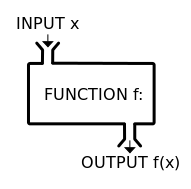
\includegraphics[width=.2\textwidth]{function.png}
 % \caption*{}
\end{figure}
\item To express that $f$ is a function from $A$ to $B$, we write 
\[ f:A \to B\]
\item We can evaluate $f$ at any element $a \in A$ to get its \emph{value} or \emph{output} $f(a)$. This is read ``$f$ of a".

\end{itemize}
}

\frame
{
\frametitle{Math - Special Functions}
\begin{itemize}[<+->]
\item Powers of x 
\begin{figure}
  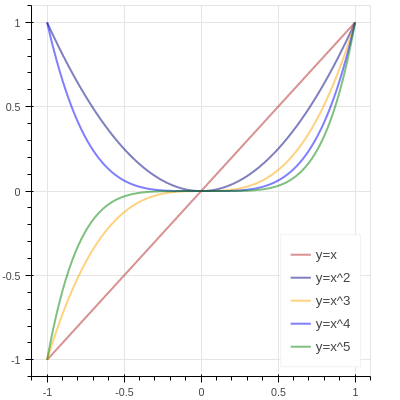
\includegraphics[width=.3\textwidth]{powers.png}
 % \caption*{}
\end{figure}
\item Trig functions 
\begin{figure}
  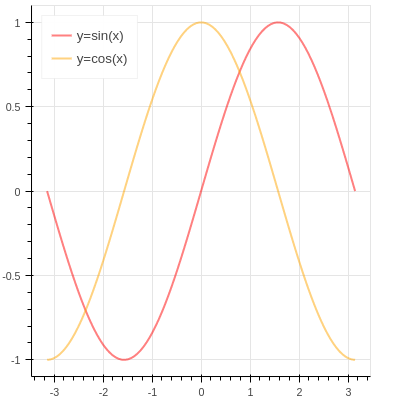
\includegraphics[width=.3\textwidth]{trig.png}
 % \caption*{}
\end{figure}
\end{itemize}
}

\frame
{
\frametitle{Math - Special Functions}
\begin{itemize}[<+->]
\item The exponential function
\begin{figure}
  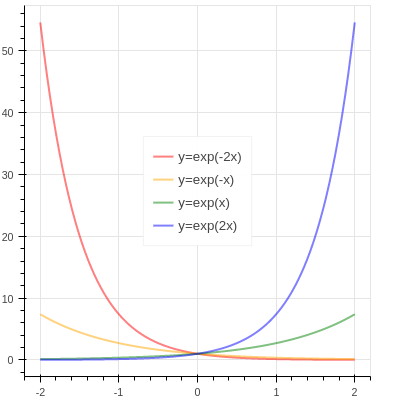
\includegraphics[width=.3\textwidth]{expon.png}
 % \caption*{}
\end{figure}
\item Sigmoids 
\begin{figure}
  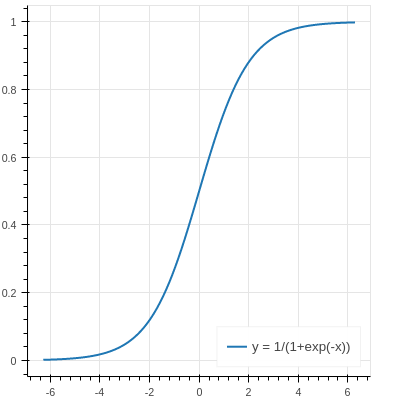
\includegraphics[width=.3\textwidth]{sigmoid.png}
 % \caption*{}
\end{figure}
\item Piecewise functions
\item Gaussians
\end{itemize}
}

\frame
{
\frametitle{Math - Special Functions}
\begin{itemize}[<+->]
\item Piecewise functions
\begin{figure}
  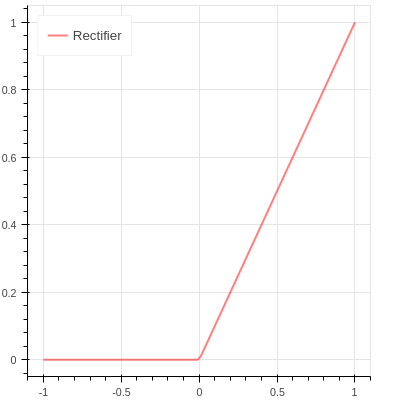
\includegraphics[width=.3\textwidth]{rectifier.png}
 % \caption*{}
\end{figure}
\item Gaussians
\begin{figure}
  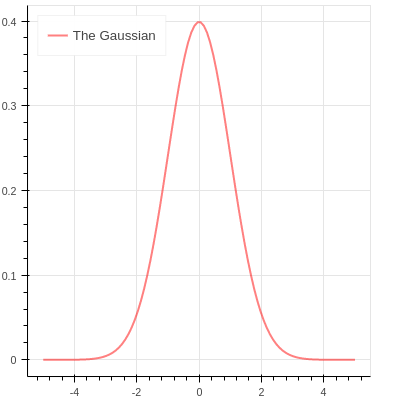
\includegraphics[width=.3\textwidth]{gaussian.png}
 % \caption*{}
\end{figure}
\end{itemize}
}

\frame
{
\frametitle{Math - Matrices \& Vectors}
\begin{itemize}[<+->]
\item A vector $v \in \R^n$ is a column of values, indexed from $1$ to $n$
\[ 
\begin{pmatrix}
v_1  \\
\vdots  \\
v_n  \\
\end{pmatrix}
\]
\item Example 
\[ 
\begin{pmatrix}
1\\
2\\
-1\\
\end{pmatrix}
\in \R^3
\]
\end{itemize}
}

\frame
{
\frametitle{Math - Matrices \& Vectors}
\begin{itemize}[<+->]
\item We can add vectors $v,w \in \R^n$. The $i^{th}$ entry $(v+w)_i$ of the sum $v+w$ is the sum of the $i^{th}$ entries of $v$ and $w$.
\item Example 
\[ 
\begin{pmatrix}
1\\
2\\
-1\\
\end{pmatrix}
+
\begin{pmatrix}
3\\
0\\
8\\
\end{pmatrix}
=
\begin{pmatrix}
4\\
2\\
7\\
\end{pmatrix}
\]
\end{itemize}
}

\frame
{
\frametitle{Math - Matrices \& Vectors}
\begin{itemize}[<+->]
\item We can compute the \emph{dot product} $v \cdot w$ of vectors $v,w \in \R^n$, defined as the sum of the pairwise products of the entries of $v$ and $w$. 
\item Example 
\[ 
\begin{pmatrix}
1\\
2\\
-1\\
\end{pmatrix}
\cdot
\begin{pmatrix}
3\\
0\\
8\\
\end{pmatrix}
=
-5
\]
\end{itemize}
}

\frame
{
\frametitle{Math - Matrices \& Vectors}
\begin{itemize}[<+->]
\item A matrix is a rectangular grid of numbers. The space of real $n\times m$ matrices is denoted $M_{n,m}(\R)$. 
\item You can think of it as a sequence of columns, or a stack of rows 
\item Example (we saw it yesterday)
\[
A = 
\begin{pmatrix}
1 & 1 & 0 \\
0 & 1 & 1 \\
0 & 0 & 2 \\
\end{pmatrix}
\]
\item The entry in the $i^{th}$ row and $j^{th}$ column of the matrix $A$ is denoted $A_{i,j}$. What is $A_{2,2}$?
\end{itemize}
}

\frame
{
\frametitle{Math - Matrices \& Vectors}
\begin{itemize}[<+->]
\item We can multiply a vector by a matrix. 
\item Matrices in $M_{n,m}(\R)$ can be multiplied on the left with vectors in $\R^m$.
\item The $i^{th}$ entry of the product $Av$ is the dot product of $v$ with the $i^{th}$ row of $A$.
\item Example 
\[
\begin{pmatrix}
1 & 1 & 0 \\
0 & 1 & 1 \\
0 & 0 & 2 \\
\end{pmatrix}
\begin{pmatrix}
1\\
2\\
-1\\
\end{pmatrix}
=
\begin{pmatrix}
3\\
1\\
-2\\
\end{pmatrix}
\]
\item This means that matrix multiplication is a \emph{function}! 
\end{itemize}
}

\frame
{
\frametitle{Math - Matrices \& Vectors}
\begin{itemize}[<+->]
\item The matrix and vector below have a special relationship - what is it? 
\[
\begin{pmatrix}
1 & 1 & 0 \\
0 & 1 & 1 \\
0 & 0 & 2 \\
\end{pmatrix}
\begin{pmatrix}
1\\
0\\
0\\
\end{pmatrix}
=
\begin{pmatrix}
1\\
0\\
0\\
\end{pmatrix}
\]
\item The vector above is an \emph{eigenvector} of the matrix corresponding to the \emph{eigenvalue} $1$.
\item Generally, a nonzero vector $v$ is an eigenvector of the matrix $A$ with eigenvalue $\lambda$ if
\[ Av = \lambda v\] 
\item Let's find some other eigenvectors.
\end{itemize}
}

\frame
{
\frametitle{Math - Stats}
\begin{itemize}[<+->]
\item A probability distribution is a function assigning a probability to each of a set of possible outcomes.
\item The distribution is everywhere nonnegative.
\item It must sum or integrate to $1$ over the entire domain of possible outcomes.
\item Examples include the uniform, normal and Poisson distributions.
\item A \emph{cumulative distribution function} gives the probability of all univariate outcomes up to and including the given value.
\end{itemize}
}

\frame
{
\frametitle{Math - Stats}
Example \\
\begin{figure}
  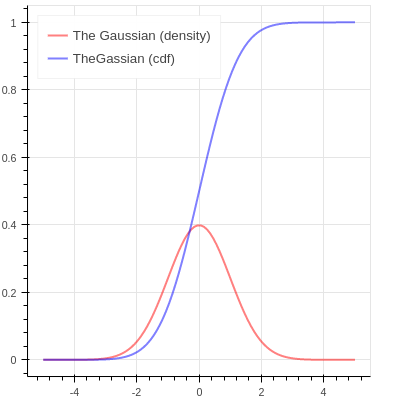
\includegraphics[width=.4\textwidth]{gaussian_cdf.png}
\end{figure}
}

\end{document} 
